\chapter{Background}\label{C:backgroundsurvey}
This chapter presents concepts related to the study conducted in this report. After each idea is introduced and discussed the relation to this work is explored.

\section{Intepretability}
To create a system that is interpretable it is necessary to have an understanding of what it means to interpret a model and how its interpretation might be evaluated. Intepretability of Machine Learning systems has been defined as \textit{"the ability to explain or to present in understandable terms"} \cite{doshi2017towards} which is ambiguous.\\

When is an interpretable model necessary? \cite{doshi2017towards} In some problem domains there is no risk associated with incorrect answers, in this situation there may be less interest a model which can be interpreted.\\

Problem domains where there is a high risk associated with incorrect answers include Safety and Ethics. A survey, "Concrete Problems in AI Safety" \cite{amodei2016concrete} provides an example of potential safety issues with AI in the context of a cleaning robot.  For example if the robot's objective is to have a known environment containing no mess, how can the robot be prevented from disabling its sensors which it uses to detect the mess?\\

It has been demonstrated that Machine Learning systems learn human like biases from textual data \cite{caliskan2017semantics}. A study done in 2010 \cite{ruggieri2010data} developed a method to analyse datasets for biases against particular classes of people. Analysis was conducted on the \textit{German Credit Dataset} which showed that discriminatory decisions where hidden in the data. An ANN trained on this data could learn these underlying biases. If the model was interpretable then it could be examined for discriminatory patterns.\\

If an ANN model is presented as being interpretable how can this be verified in a scientific way? There are three categories of evaluation techniques \cite{doshi2017towards}.

\comment{The titles are from another paper but descriptions are in my own words. Improve description here}
\begin{enumerate}
	\item \textit{"Application-Grounded Evaluation"} Conducting experiments with human subjects in a specific problem domain. If the goal is to learn an interpretable classifier to grant bank loans then a domain expert in granting/denying loans should be used to establish intepretability.
	
	\item \textit{"Human-Grounded Metrics"} Designing simpler experiments which still allow for establishing intepretability in a specific domain. This situation occurs when access to domain experts is either to expensive or difficult. The tasks can be simplified to allow humans that are not domain experts to complete them.
	
	\item \textit{"Functionally-Grounded Evaluation"} If it is possible to define intepretability in terms of the problem then it can be used to establish this property in the model.
\end{enumerate}

\subsection{Relation to Solution}
The report is presenting an interpretable model. Consequently it is important to understand what it means for a model to be interpretable and how this property can be evaluated in the solution presented.


\section{Rule Extraction}

A survey in 1995 focuses on rule extraction algorithms \cite{andrews1995survey}, identifying the reasons for needing these algorithms along with introducing ways to categorise and compare them.\\

There are three categories that rule extraction algorithms fall into \cite{andrews1995survey}. An algorithm in the \textbf{decompositional} category focuses on extracting rules from each hidden/output unit. If an algorithm is in the \textbf{pedagogical} category then rule extraction is thought of as a learning process. The ANN is treated as a black box and the algorithm learns a relationship between the input and output vectors. The third category, \textbf{electic}, is a combination of decompositional and pedagogical. An Electic algorithm inspects the hidden/output neurons individually but extracts rules which represent the ANN globally \cite{tickle1998truth}.\\

To further divide the categories two more distinctions are introduced. One measures the portability of rule extraction techniques, i.e. how easily can they be applied to different types of ANN's? The second is criteria to assess the quality of the extracted rules, these are accuracy, fidelity, consistency, comprehensibility \cite{andrews1995survey}.

\begin{enumerate}
\item A rule set is \textbf{Accurate} if it can generalize, i.e. classify previously unseen examples.
\item The behaviour of a rule set with a high \textbf{fedelity} is close to that of the ANN it was extracted from.
\item A rule set is \textbf{consistent} if when trained under different conditions it generates rules which assign the same classifications to unseen examples.
\item The measure of \textbf{comprehensibility} is defined by the number of rules in the set and the number of literals per rule.
\end{enumerate}

\subsection{Relation to Solution}
These survayes provide a framework for evaluating the rules extracted using a particular technequic. The solution developed in this report allows for rule exaction in some situations. By introducing this content the reader is familiar with this approach to evaluating extracted rule sets.

Rule extraction algorithms make up a large portion of the current methods to interpret knowledge inside an ANN.

\section{LIME: Local Interpretable Model-Agnostic Explanations}
\comment{Prehapse add more here?}
The paper "'Why should I Trust You?' Explaining the Predictions of Any Classifier" \cite{ribeiro2016should} published in 2016 presents a novel approach to interpretation of Machine Learning models. The motivation for this research is the idea of trusting the answers provided, either in the context of an individual prediction or the model as a whole. The LIME technequic provides an explanation of a single prediction. Trust in the model can be developed by inspecting explanations of many individual predictions.

\subsection{Relation to Solution}
LIME is a recent and effect method for interpreting models. Consequently it will provide an effective benchmark for comparing the solution presented in this report.

\section{Noisy Neurons} \label{sec:background-noisy-neurons}
Multi-Layer Perceptron Networks (MLPNs) are universal function approximators \cite{hornik1989multilayer}, as such can achieve a high accuracy across a broad range of problems. \hl{There are many equivalent weight representations of an MLPN which give the same solutions}, this makes interpreting the network difficult \cite{LearningLogicalActivations}. By restricting the possible relationships between a neurons inputs and outputs to be a single function then only the relevance of each feature needs to be inferred. Consequently the problem interpretation becomes easier. The two functions OR and AND are easy to understand, which is a good reason to pick them over other functions.\\

In 2016 the concept of Noisy-OR and Noisy-AND neurons \cite{LearningLogicalActivations} where derived from the Noisy-OR relation \cite{russell1995modern}, a concept in Bayesian Networks developed by Judea Pearl. A Bayesian Network represents the conditional dependencies between random variables in the form of a directed acyclic graph \cite{neapolitan2004learning}.

\begin{figure}[H]
	\centering
	\begin{minipage}[b]{0.4\textwidth}
		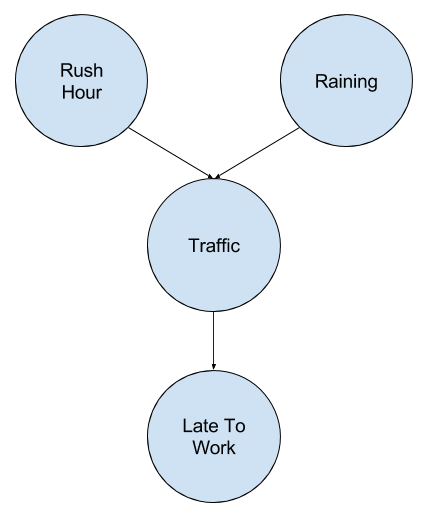
\includegraphics[width=\textwidth]{bayesian-network-example.png}
		\caption{}
		\label{fig:bayesian-network-example}
	\end{minipage}
	\hfill
\end{figure}

Figure \ref{fig:bayesian-network-example} is a Bayesian network. It demonstrates the dependency between random variables "Rush Hour", "Raining", "Traffic", "Late To Work". The connections show dependencies i.e. Traffic influences whether you are late to work,\ and it being rush hour or raining influences whether there is traffic.\\

Consider a Bayesian Network with a node $D$ and $S_1,..., S_n$ being $D$s parents. In other words $S_i$ influences the node $D$. Each $S_i$ is independent from all others. The relationship between D and its parents is defined as if $S_1\ OR\ ...\ OR\ S_n$ is true then $D$ is true. This relationship is binary but there might be uncertantly as to whether each parent influences the child. Let $\epsilon_i$ be the uncertainty that $S_i$ influence $D$. If $\epsilon_i = 0$ then parent $i$ influences the child, otherwise if $\epsilon_i = 1$ it does not. Therefore $P(D = 1| S_1 = 1, , S_n = 1)$ can be defined as Equation \ref{equ:noisy-or-relation}. Given all the parents are 1, if the child is influenced by at least one of its parents then $\prod^n_{i=1} \epsilon_i = 0$ and it is on. On the other hand if it is not influenced by any of its parents then $\prod^n_{i=1} \epsilon_i = 1$ so it is off.

\begin{align}
P(D = 1 | S_1 = 1, ..., S_n = 1) = 1 - \prod^n_{i=1} \epsilon_i
\label{equ:noisy-or-relation}
\end{align}

Equation \ref{equ:noisy-or-relation} shows the noisy or relation. In the context of a neuron the inputs $x_1, ..., x_n$ represent the probability that inputs $1, ..., n$ are true. The output of a neuron as conditionally dependent on its inputs, in terms of a Bayesian Network the $x_i$'s is a parent of the neuron. Each $\epsilon_i$ is the uncertainty as to whether $x_i$ influences the neurons output. How can weights and inputs be combined to create a final activation value for the neuron? First consider a function $f(\epsilon, x)$ which computes the irrelevance of input x. Some conditions \cite{LearningLogicalActivations} that can be placed on $f$ are given in the following list. 

\begin{enumerate}
	\item $\epsilon = 1$ means that $f(\epsilon, x) = 1$
	\item $x = 1$ means that $f(\epsilon, x) = 1$
	\item Monotonically increasing in $\epsilon$ and decreasing in x. Let $f(x, \epsilon) = \epsilon^x$. The definitions for Noisy-OR and Noisy-AND gates can now be given.
\end{enumerate}

The function $f(\epsilon, x)$ is 1 (i.e x is irrelevant) if x does not influence the output ($\epsilon = 1$) essentially cancelling these irrelevant inputs out in a AND or OR. The noisy activations can therefore be a logical function over $f(\epsilon_{x_i}, x_i)$ for all $i$.

\begin{definition}
	A \textbf{Noisy-OR} Neuron has weights $\epsilon_1, ..., \epsilon_n \in (0,1]$ which represent the uncertainty that corresponding inputs $x_1, ..., x_n \in [0,1]$ influence the output. The activation of a Noisy-OR Neurons is given in Equation \ref{equ:noisy-or-activation-1}.
	
	\begin{align}
	a = 1 - \prod^p_{i=1} (\epsilon_i^{x_i}) \cdot \epsilon_b
	\label{equ:noisy-or-activation-1}
	\end{align}
\end{definition}

\begin{definition}
	A \textbf{Noisy-AND} Neuron has weights $\epsilon_1, ..., \epsilon_n \in (0, 1]$ which represent the uncertainty that corresponding inputs $x_1, ..., x_n \in [0,1]$ influence the output. The activation of a Noisy-AND Neurons is given in Equation \ref{equ:noisy-and-activation-1}
	
	\begin{align}
	a = \prod^p_{i=1} (\epsilon_i^{1 - x_i}) \cdot \epsilon_b
	\label{equ:noisy-and-activation-1}
	\end{align}
\end{definition}

Both these parametrisations reduce to discrete logic gates when there is no noise, i.e. $\epsilon_i = 0$ for all $i$.\\

\subsection{Relation to Solution}
The noisy neurons are the building blocks for the two network architectures present in this report. Without an understanding of these concepts it would be difficult to understand the motivations for the solution developed.

\section{Logical Normal Form Networks}
\subsection{CNF \& DNF}
A boolean formula is in Conjunctive Normal Form (CNF) if and only if it is a conjunction (and) of clauses. A clause in a CNF formula is given by a disjunction (or ) of literals. A literal is either an atom or the negation of an atom, an atom is one of the variables in the formula.\\

Consider the boolean formula $\lnot a \lor (b \land c)$, the CNF is $(\lnot a \lor b) \land (\lnot a \lor c)$. In this CNF formula the clauses are $(\lnot a \lor b)$, $(\lnot a \lor c)$, the literals used are $\lnot a$, $b$, $c$ and the atoms are $a$, $b$, $c$.\\

A boolean formula is in Disjunctive Normal Form (DNF) if and only if it is a disjunction (or) of clauses. A DNF clause is a conjunction (and) of literals. Literals and atoms are defined the same as in CNF formulas.\\

Consider the boolean formula $\lnot a \land (b \lor c)$, the DNF is $(\lnot a \land b) \lor (\lnot a \land c)$.\\

\subsection{CNF \& DNF from Truth Table} \label{subsec:construct-cnfdnf}
Given a truth table representing a boolean formula, constructing a DNF formula involves taking all rows which correspond to True and combining them with an OR operation. To construct a CNF one combines the negation of any row which corresponds to False by an OR operation and negates it.

\begin{theorem}
	The maximum number of clauses in a CNF or DNF formula is $2^n$
	\label{thm:max-clause-cnfdnf}
\end{theorem}

\begin{proof}
	Assume the goal is to find the CNF and DNF for a Boolean formula B of size $n$, for which the complete truth table is given. The truth table has exactly $2^n$ rows.\\
	
	First assume a CNF is being constructed, this is achieved by taking the OR of the negation of all rows corresponding to False, the NOT operation leaves the number of clauses unchanged. At most there can be $2^n$ rows corresponding to False, consequently there are at most $2^n$ clauses in the CNF.\\
	
	A similar argument shows that the same holds for DNF.
\end{proof}

\subsection{Definition of Logical Normal Form Networks}
In 1996 a class of networks called Logical Normal Form Networks \cite{herrmann1996backpropagation} (LNFNs) where developed. Focusing on learning the underlying CNF or DNF for a boolean expression which describes the problem. The approach relies on a specific network configuration along with restriction the function space of each neuron, allowing them to only perform an OR or AND on a subset of their inputs. Such OR and AND neurons are called Disjunctive and Conjunctive retrospectively. If the trained network is able to achieve a low enough accuracy then rules can be extracted from the network in terms of a Boolean CNF or DNF expression \cite{herrmann1996backpropagation}.\\

The algorithm which extracts rules from LNFNs would be Electic and certainly is not Portable as the algorithm is specific to the LNFN architecture. It is not possible to further classify the rule extraction algorithm as the research developing it lacks any experimental results. Justification is also missing making the LNFNs difficult to reproduce.\\

\subsection{Relation to Solution}
The motivation for the development of the solution presented in this report (Logical Neural Networks) can be derived as a more flexable version of Logical Normal Form Networks.

\section{Logical Neural Networks}
ANN's containing of Noisy-OR and Noisy-AND neurons are called Logical Neural Networks \cite{LearningLogicalActivations} (LNN's). If the network consists of only Noisy neurons then it a pure LNN. ANNs containing a mix of logical and standard activations where shown to not yield interpretable models and also have lower performance, consequently when LNNs are refered to it will always be in the context of Pure LNNs.

\subsection{Relation to Solution}
The solution presented is a modified Logical Neural Network structure.
